%\documentclass[landscape,a0paper,fontscale=0.292]{baposter}
\documentclass[portrait,kjemiDim,fontscale=0.292]{baposter}

\usepackage[vlined]{algorithm2e}
\usepackage{times}
\usepackage{calc}
\usepackage{url}
\usepackage{graphicx}
\usepackage{amsmath}
\usepackage{amssymb}
\usepackage{relsize}
\usepackage{multirow}
\usepackage{booktabs}

\usepackage{graphicx}
\usepackage{multicol}
\usepackage[T1]{fontenc}
\usepackage{ae}
\usepackage{color}
\usepackage{wrapfig}
\usepackage{multirow}

\graphicspath{{images/}}

 %%%%%%%%%%%%%%%%%%%%%%%%%%%%%%%%%%%%%%%%%%%%%%%%%%%%%%%%%%%%%%%%%%%%%%%%%%%%%%%%
 %%%% Some math symbols used in the text
 %%%%%%%%%%%%%%%%%%%%%%%%%%%%%%%%%%%%%%%%%%%%%%%%%%%%%%%%%%%%%%%%%%%%%%%%%%%%%%%%
 % Format 
 \newcommand{\RotUP}[1]{\begin{sideways}#1\end{sideways}}


 %%%%%%%%%%%%%%%%%%%%%%%%%%%%%%%%%%%%%%%%%%%%%%%%%%%%%%%%%%%%%%%%%%%%%%%%%%%%%%%%
 % Multicol Settings
 %%%%%%%%%%%%%%%%%%%%%%%%%%%%%%%%%%%%%%%%%%%%%%%%%%%%%%%%%%%%%%%%%%%%%%%%%%%%%%%%
 \setlength{\columnsep}{0.7em}
 \setlength{\columnseprule}{0mm}


 %%%%%%%%%%%%%%%%%%%%%%%%%%%%%%%%%%%%%%%%%%%%%%%%%%%%%%%%%%%%%%%%%%%%%%%%%%%%%%%%
 % Save space in lists. Use this after the opening of the list
 %%%%%%%%%%%%%%%%%%%%%%%%%%%%%%%%%%%%%%%%%%%%%%%%%%%%%%%%%%%%%%%%%%%%%%%%%%%%%%%%
 \newcommand{\compresslist}{%
 \setlength{\itemsep}{1pt}%
 \setlength{\parskip}{0pt}%
 \setlength{\parsep}{0pt}%
 }


 %%%%%%%%%%%%%%%%%%%%%%%%%%%%%%%%%%%%%%%%%%%%%%%%%%%%%%%%%%%%%%%%%%%%%%%%%%%%%%
 % Formating
 \newcommand{\Matrix}[1]{\begin{bmatrix} #1 \end{bmatrix}}
 \newcommand{\Vector}[1]{\begin{pmatrix} #1 \end{pmatrix}}

 \newcommand*{\norm}[1]{\mathopen\| #1 \mathclose\|}% use instead of $\|x\|$
 \newcommand*{\abs}[1]{\mathopen| #1 \mathclose|}% use instead of $\|x\|$
 \newcommand*{\normLR}[1]{\left\| #1 \right\|}% use instead of $\|x\|$

 \newcommand*{\SET}[1]  {\ensuremath{\mathcal{#1}}}
 \newcommand*{\FUN}[1]  {\ensuremath{\mathcal{#1}}}
 \newcommand*{\MAT}[1]  {\ensuremath{\boldsymbol{#1}}}
 \newcommand*{\VEC}[1]  {\ensuremath{\boldsymbol{#1}}}
 \newcommand*{\CONST}[1]{\ensuremath{\mathit{#1}}}

 \DeclareMathOperator*{\argmax}{arg\,max}
 \DeclareMathOperator*{\diag}{diag}
 \DeclareMathOperator*{\argmin}{arg\,min}
 \DeclareMathOperator*{\vectorize}{vec}
 \DeclareMathOperator*{\reshape}{reshape}

 %-----------------------------------------------------------------------------
 % Differentiation
 \newcommand*{\Nabla}[1]{\nabla_{\!#1}}

 \renewcommand*{\d}{\mathrm{d}}
 \newcommand*{\dd}{\partial}

 \newcommand*{\At}[2]{\ensuremath{\left.#1\right|_{#2}}}
 \newcommand*{\AtZero}[1]{\At{#1}{\pp=\VEC 0}}

 \newcommand*{\diffp}[2]{\ensuremath{\frac{\dd #1}{\dd #2}}}
 \newcommand*{\diffpp}[3]{\ensuremath{\frac{\dd^2 #1}{\dd #2 \dd #3}}}
 \newcommand*{\diffppp}[4]{\ensuremath{\frac{\dd^3 #1}{\dd #2 \dd #3 \dd #4}}}
 \newcommand*{\difff}[2]{\ensuremath{\frac{\d #1}{\d #2}}}
 \newcommand*{\diffff}[3]{\ensuremath{\frac{\d^2 #1}{\d #2 \d #3}}}
 \newcommand*{\difffp}[3]{\ensuremath{\frac{\dd\d #1}{\d #2 \dd #3}}}
 \newcommand*{\difffpp}[4]{\ensuremath{\frac{\dd^2\d #1}{\d #2 \dd #3 \dd #4}}}

 \newcommand*{\diffpAtZero}[2]{\ensuremath{\AtZero{\diffp{#1}{#2}}}}
 \newcommand*{\diffppAtZero}[3]{\ensuremath{\AtZero{\diffpp{#1}{#2}{#3}}}}
 \newcommand*{\difffAt}[3]{\ensuremath{\At{\difff{#1}{#2}}{#3}}}
 \newcommand*{\difffAtZero}[2]{\ensuremath{\AtZero{\difff{#1}{#2}}}}
 \newcommand*{\difffpAtZero}[3]{\ensuremath{\AtZero{\difffp{#1}{#2}{#3}}}}
 \newcommand*{\difffppAtZero}[4]{\ensuremath{\AtZero{\difffpp{#1}{#2}{#3}{#4}}}}

 %-----------------------------------------------------------------------------
 % Defined
 % How should the defined operator look like (:= or ^= ==)
 % (I want back my :=, it is so much better than ^= because (1) it has a
 % direction and (2) everyone here uses it.)
 %
 % Use :=
 %\newcommand*{\defined}{\ensuremath{\mathrel{\mathop{:}}=}}
 %\newcommand*{\definedRight}{\ensuremath{=\mathrel{\mathop{:}}}}
 % Use ^=
 \newcommand*{\defined}{\ensuremath{\triangleq}}
 \newcommand*{\definedRight}{\ensuremath{\triangleq}}
 % Use = with three bars
 %\newcommand*{\defined}{\ensuremath{?}}
 %\newcommand*{\definedRight}{\ensuremath{?}}

 %%%%%%%%%%%%%%%%%%%%%%%%%%%%%%%%%%%%%%%%%%%%%%%%%%%%%%%%%%%%%%%%%%%%%%%%%%%%%%
 % Symbols used in the paper

 %-----------------------------------------------------------------------------
 % The Methods
 \newcommand*{\ICIA}{\emph{ICIA}}
 \newcommand*{\CoDe}{\emph{CoDe}}
 \newcommand*{\LinCoDe}{\emph{LinCoDe}}
 \newcommand*{\CoNe}{\emph{CoNe}}
 \newcommand*{\CoLiNe}{\emph{CoLiNe}}
 \newcommand*{\LinCoLiNe}{\emph{LinCoLiNe}}

 % inter eye distance
 \newcommand*{\ied}{IED}

 %-----------------------------------------------------------------------------
 % Koerper
 %%\newcommand*{\RR}{\mathbb{R}}
 %\newcommand*{\RR}{{I\hspace{-3.5pt}R}}
 %\newcommand*{\RR}{{\mathrm{I\hspace{-2.7pt}R}}}

 \font\dsfnt=dsrom12

 \DeclareSymbolFont{nark}{U}{dsrom}{m}{n}
 \DeclareMathSymbol{\NN}{\dsfnt}{nark}{`N}
 \DeclareMathSymbol{\RR}{\dsfnt}{nark}{`R}
 \DeclareMathSymbol{\ZZ}{\dsfnt}{nark}{`Z}

 %-----------------------------------------------------------------------------
 % Domains
 \newcommand*{\D}{\mathcal{D}}
 \newcommand*{\I}{\mathcal{I}}

 %-----------------------------------------------------------------------------
 % Texture coordinates
 \newcommand*{\rr}{\VEC{r}}

 %-----------------------------------------------------------------------------
 % Parameters
 \newcommand*{\pt}{\VEC{\tau}}
 \newcommand*{\pr}{\VEC{\rho}}
 \newcommand*{\pp}{\VEC{p}}
 \newcommand*{\qq}{\VEC{q}}
 \newcommand*{\xx}{\VEC{x}}
 \newcommand*{\deltaq}{\Delta \qq}
 \newcommand*{\deltap}{\Delta \pp}
 \newcommand*{\zz}{\VEC{z}}
 \newcommand*{\pa}{\VEC{\alpha}}
 \newcommand*{\qa}{\VEC{\alpha}}
 \newcommand*{\pb}{\VEC{\beta}}

 %-----------------------------------------------------------------------------
 % Optimal appearance parameters
 \newcommand*{\pbh}[1]{\ensuremath{\hat{\pb}({#1})}}

 %-----------------------------------------------------------------------------
 % Warp basis
 \newcommand*{\M}[1]{\ensuremath{M({#1})}}
 \newcommand*{\LL}[1]{\ensuremath{L({#1})}}

 %-----------------------------------------------------------------------------
 % Matrices of the texture model
 \newcommand*{\AM}[1]{\ensuremath{\Lambda(#1)}}               % Lambda(beta) 
 \newcommand*{\AMr}[2]{\ensuremath{\Lambda(#1; #2)}}        % Lambda(r, beta)

 \newcommand*{\As}{A}         % Continuous Basis symbol
 \newcommand*{\afs}{a}        % Continuous mean symbol
 \newcommand*{\A}[1]{\As(#1)}         % Continuous Basis
 \newcommand*{\af}[1]{\afs(#1)}        % Continuous mean


 %-----------------------------------------------------------------------------
 % Matrices of the shape model
 \newcommand*{\MU}{\VEC{\mu}}
 \newcommand*{\MM}{\MAT{M}}

 %-----------------------------------------------------------------------------
 %% The project out matrix and operator
 \newcommand*{\INT}{\MAT{P}}
 \newcommand*{\INTf}{P}

 %-----------------------------------------------------------------------------
 % The identity matrix
 \newcommand*{\EYEtwo}{\Matrix{1 & 0\\0&1}}
 \newcommand*{\EYE}{\MAT E}
 \newcommand*{\EYEf}{E}

 % Wether to use subscripts or brackets for some function arguments
 % can be decided by commenting out the corresponding functions underneath
 %-----------------------------------------------------------------------------
 % Mapping
 \newcommand*{\Cs}[1]{\ensuremath{C^{#1}}} % C symbol
 \newcommand*{\C}[2]{\ensuremath{C^{#1}(#2)}} % Use C with brackets

 %-----------------------------------------------------------------------------
 % Objective function
 \newcommand*{\Fs}{\ensuremath{F}}              % F symbol
 \newcommand*{\F}[1]{\ensuremath{\Fs(#1)}}       % Use F with brackets    F(q)

 %-----------------------------------------------------------------------------
 % Approximated objective functions
 \newcommand*{\FFs}{\tilde{F}}                     % ~F symbol
 \newcommand*{\FF}[1]{\ensuremath{\FFs(#1)}}       % Use ~F with brackets    F(q)

 %-----------------------------------------------------------------------------
 % residual function
 \newcommand*{\es}{\ensuremath{f}}              % R symbol

 \newcommand*{\e}[1]{\ensuremath{\es(#1)}}         % R(q)
 \newcommand*{\er}[2]{\ensuremath{\es(#1; #2)}}    % R(r; q)

 %-----------------------------------------------------------------------------
 % Approximated residual functions
 \newcommand*{\ees}{\tilde{f}}                       % ~R symbol
 \newcommand*{\ee}[1]{\ensuremath{\ees(#1)}}       % ~R(q)
 \newcommand*{\eer}[2]{\ensuremath{\ees(#2; #1)}}  % ~R(r; q)

 %-----------------------------------------------------------------------------
 % Warps
 \newcommand*{\Vs}{\ensuremath{V}}
 \newcommand*{\VLins}{\ensuremath{\Vs^{\text{Ortho}}}}
 \newcommand{\VModels}{\ensuremath{\Vs^{\text{Model}}}}
 \newcommand*{\Ws}{\ensuremath{W}}

 \newcommand{\V}[1]{\ensuremath{\Vs(#1)}}
 \newcommand{\VModel}[1]{\ensuremath{\VModels(#1)}}
 \newcommand{\Vr}[2]{\ensuremath{\Vs(#1; #2)}}
 \newcommand{\VInvr}[2]{\ensuremath{\Vs^{-1}(#1; #2)}}
 \newcommand{\VrLin}[2]{\ensuremath{\VLins(#1; #2)}}
 \newcommand{\W}[1]{\ensuremath{\Ws(#1)}}
 \newcommand{\Winv}[1]{\ensuremath{\Ws^{-1}(#1)}}
 \newcommand{\Wr}[2]{\ensuremath{\Ws(#1; #2)}}


%%%%%%%%%%%%%%%%%%%%%%%%%%%%%%%%%%%%%%%%%%%%%%%%%%%%%%%%%%%%%%%%%%%%%%%%%%%%%
%% Begin of Document
%%%%%%%%%%%%%%%%%%%%%%%%%%%%%%%%%%%%%%%%%%%%%%%%%%%%%%%%%%%%%%%%%%%%%%%%%%%%%
\begin{document}
%%%%%%%%%%%%%%%%%%%%%%%%%%%%%%%%%%%%%%%%%%%%%%%%%%%%%%%%%%%%%%%%%%%%%%%%%%%%%
%% Here starts the poster
%%---------------------------------------------------------------------------
%% Format it to your taste with the options
%%%%%%%%%%%%%%%%%%%%%%%%%%%%%%%%%%%%%%%%%%%%%%%%%%%%%%%%%%%%%%%%%%%%%%%%%%%%%
\begin{poster}{
 % Show grid to help with alignment
 grid=false,
 % Column spacing
 colspacing=0.7em,
 % Color style
 headerColorOne=cyan!20!white!90!black,
 borderColor=cyan!30!white!90!black,
 % Format of textbox
 textborder=faded,
 % Format of text header
 headerborder=open,
 headershape=roundedright,
 headershade=plain,
 background=none,
 bgColorOne=cyan!10!white,
 headerheight=0.12\textheight}
 % Eye Catcher
 {
   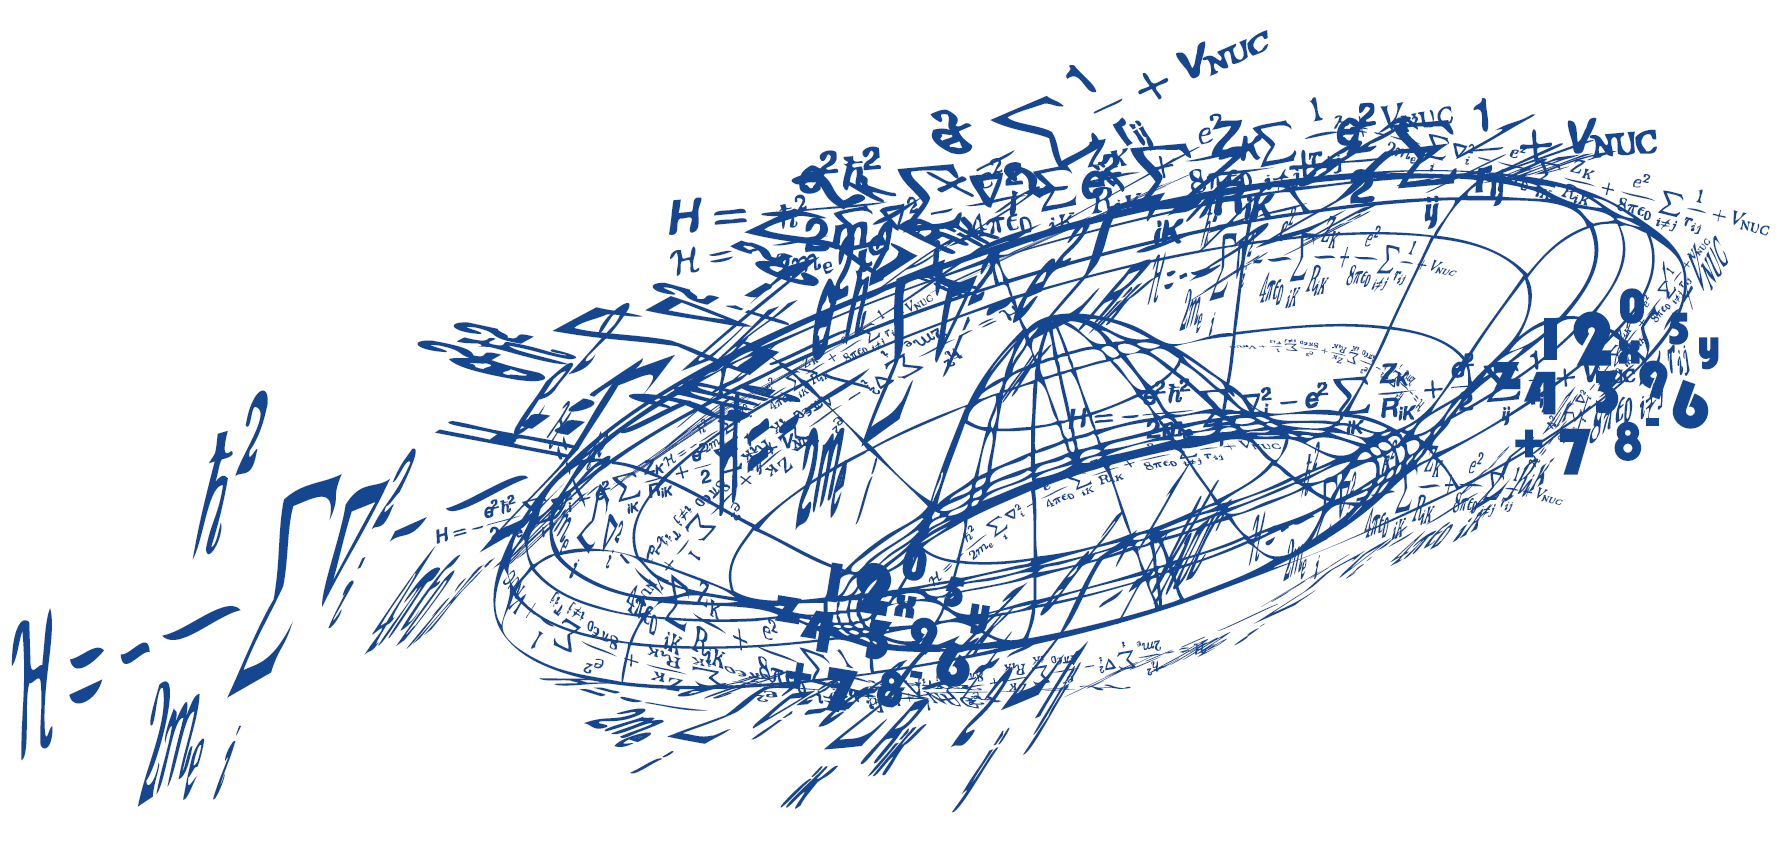
\includegraphics[width=0.3\linewidth]{ctcc-logo-blue.png} 
 }
 % Title
 {\sc\huge  Simulating  Biomolecules on Computers! }
 % Authors
 {\sc\small Patrick Merlot, Jon Austad and Johannes Rekkedal\\ %[1em]
 {\sc\tiny \texttt{patrick.merlot@kjemi.uio.no, jonaus@student.matnat.uio.no, j.a.rekkedal@kjemi.uio.no}}
 }
 % University logo
 {
  \begin{tabular}{r}
    
\includegraphics[width=0.22\linewidth]{kjemi-grand-prix-logo.jpg}\\
    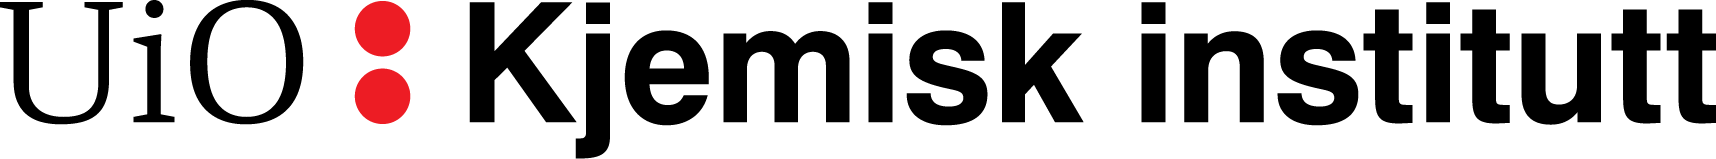
\includegraphics[width=0.22\linewidth]{logo-kjemisk-institutt-enkel.png}
  \end{tabular}
 }

%%%%%%%%%%%%%%%%%%%%%%%%%%%%%%%%%%%%%%%%%%%%%%%%%%%%%%%%%%%%%%%%%%%%%%%%%%%%%%
%%% Now define the boxes that make up the poster
%%%---------------------------------------------------------------------------
%%% Each box has a name and can be placed absolutely or relatively.
%%% The only inconvenience is that you can only specify a relative position 
%%% towards an already declared box. So if you have a box attached to the 
%%% bottom, one to the top and a third one which should be inbetween, you 
%%% have to specify the top and bottom boxes before you specify the middle 
%%% box.
%%%%%%%%%%%%%%%%%%%%%%%%%%%%%%%%%%%%%%%%%%%%%%%%%%%%%%%%%%%%%%%%%%%%%%%%%%%%%%

%%%%%%%%%%%%%%%%%%%%%%%%%%%%%%%%%%%%%%%%%%%%%%%%%%%%%%%%%%%%%%%%%%%%%%%%%%%%%%
  \headerbox{Purpose}{name=purpose,column=0,row=0,span=2}{
%%%%%%%%%%%%%%%%%%%%%%%%%%%%%%%%%%%%%%%%%%%%%%%%%%%%%%%%%%%%%%%%%%%%%%%%%%%%%%
%    \begin{multicols}{2}
    Most of physics has been known at the atomic scale for about a century.
 However simulating molecules of few thousands atoms (like important biomolecules) from first principles still requires too much computational effort.
Thanks to fast and accurate linear-scaling (LS) methods in quantum chemistry, simulating such systems may soon become routine calculations, an important step for computer-aided drug design, and more generally for bridging the gap between quantum and classical physics, e.g. between the nanoworld and our macroscopic environment.
%    \end{multicols}
  }
  %%%%%%%%%%%%%%%%%%%%%%%%%%%%%%%%%%%%%%%%%%%%%%%%%%%%%%%%%%%%%%%%%%%%%%%%%%%%%%
  \headerbox{Introduction}{name=abstract,column=0,below=purpose,span=1}{
    %%%%%%%%%%%%%%%%%%%%%%%%%%%%%%%%%%%%%%%%%%%%%%%%%%%%%%%%%%%%%%%%%%%%%%%%%%%%%%
The laws of physics at the atomic level are governed by the  \textbf{Schr\"odinger equation},
  \begin{align*}
{ \color{blue}    i\hbar\frac{\partial\psi}{\partial t} = \frac{\hbar^2}{2m}\nabla^2\psi + V(\mathbf{r})\psi }
%      \F{\qq} &\defined \normLR{ \e{\qq,\pb} }^2_{\D},\label{eqn:f}\\
    %    \text{with }  \e{\qq} &\defined a - I\circ \W{\qq}\nonumber
  \end{align*}
 with analytical solutions known for very few and small systems.% such as the hydrogen atom or the particle in a box. 

\textbf{By approximating the solutions of this equation, computational chemistry aims at predicting molecular properties, dynamics and reactions on computers}.


     \begin{tabular}{rl}
  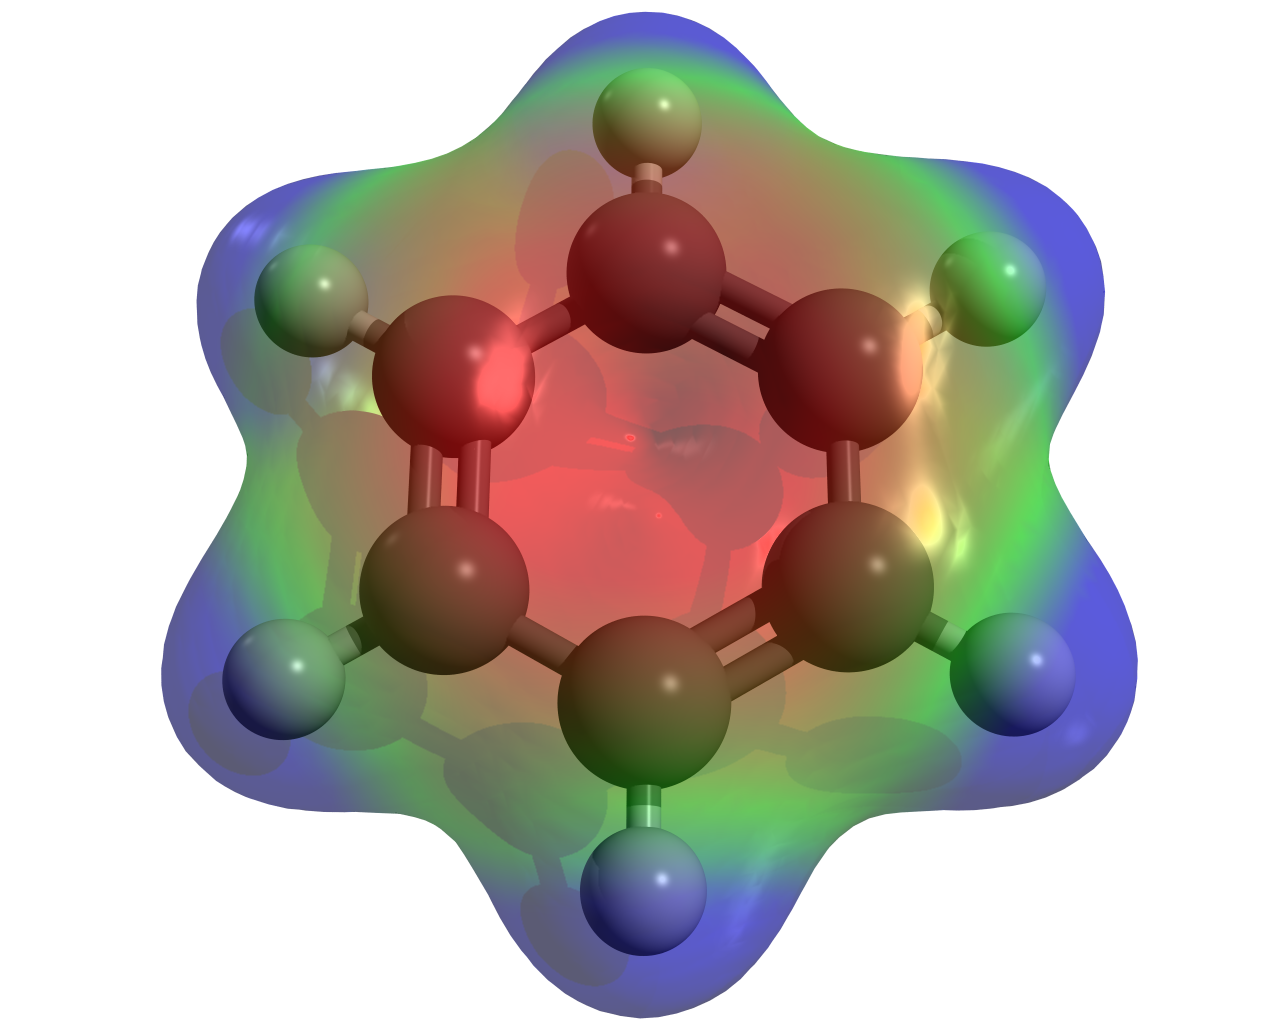
\includegraphics[scale=0.06]{benzene-density-esp1.png} &   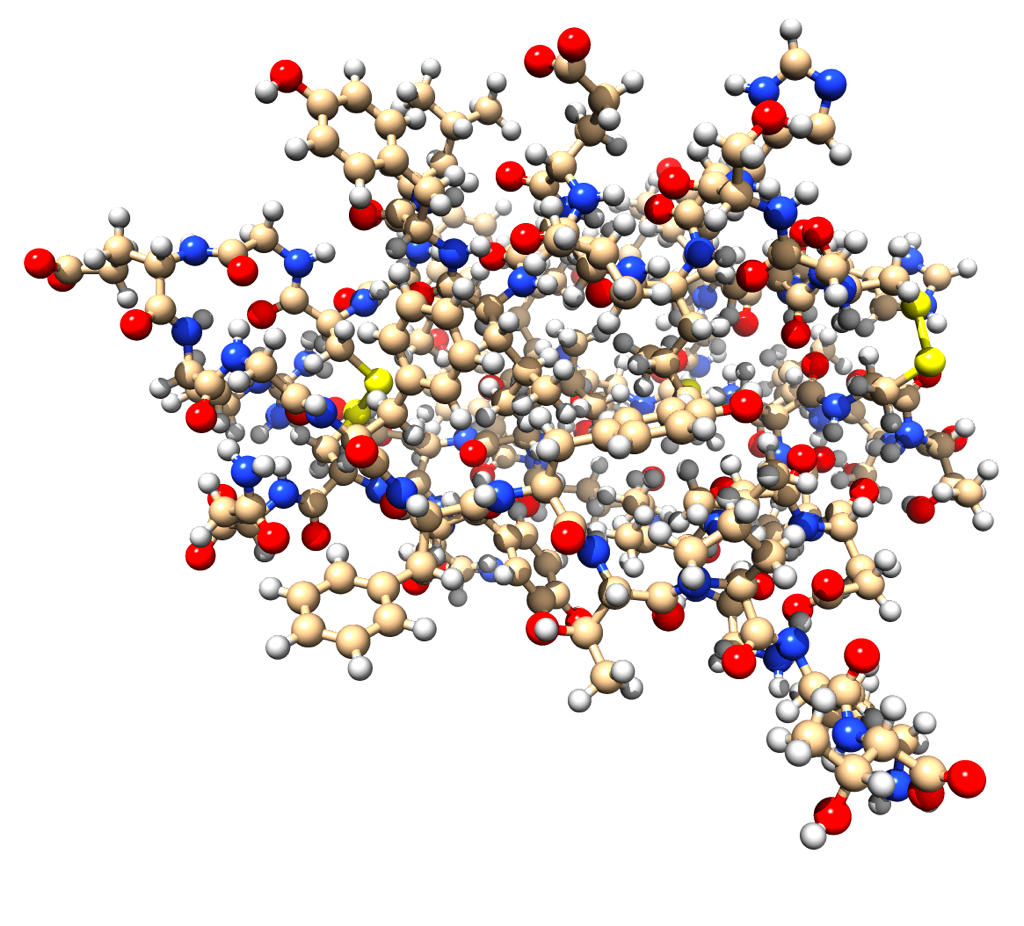
\includegraphics[scale=0.08]{insulin_TKJ.png} \\
       \end{tabular}



  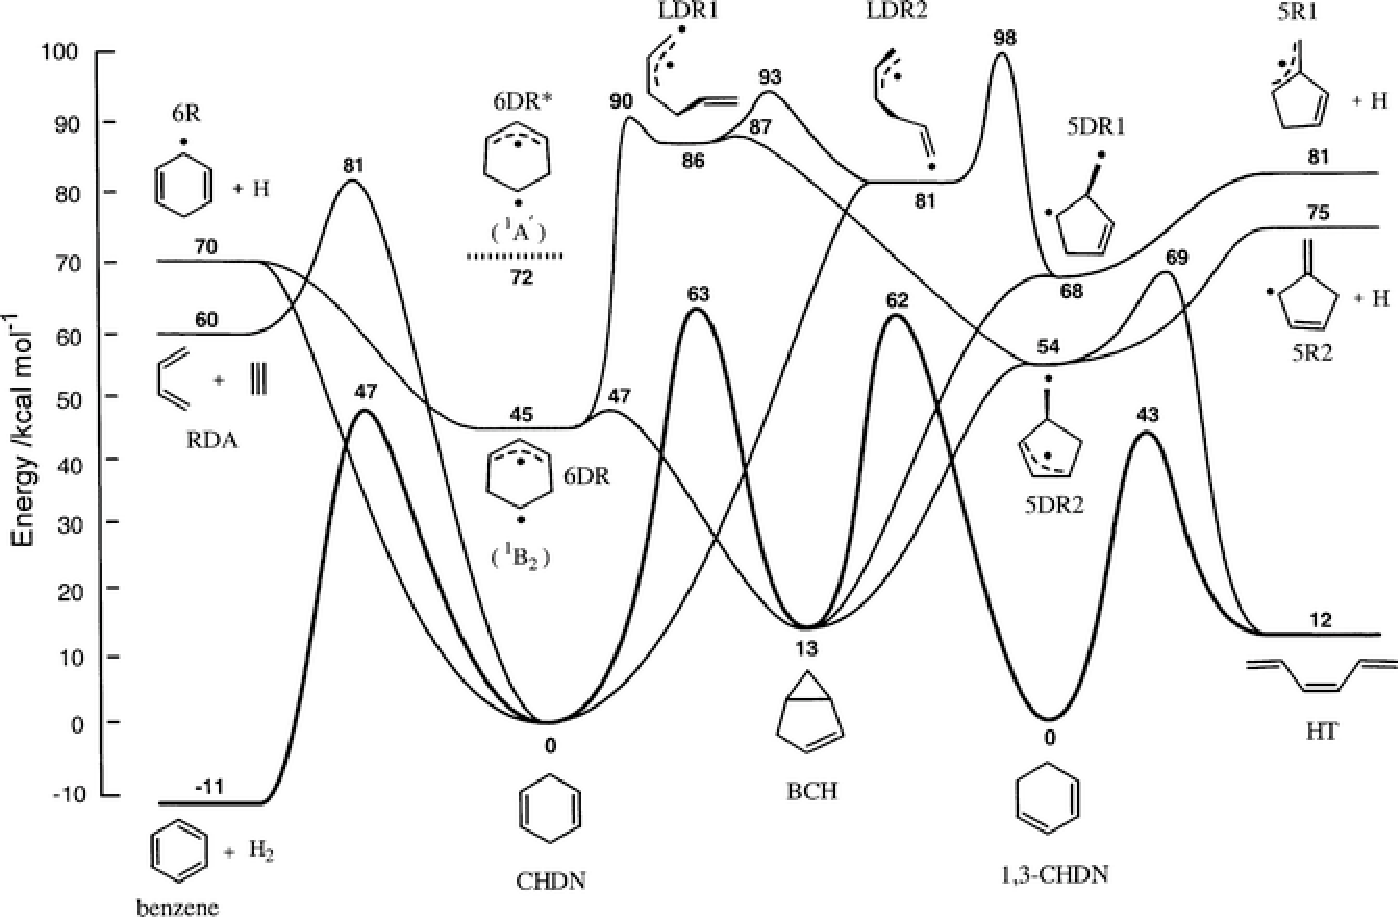
\includegraphics[scale=0.25]{DFT_reactionPathways.pdf} \\

Today about one third of the publications in chemistry uses computation to perform verifications, interpretations of experiments or even predictions.

For molecular systems with more than one electron, \textbf{a hierarchy of quantum mechanical (QM) methods allows for a systematic approach to the exact solution}, providing reliable ``measurements'' or estimations when based on the simplest approximations.


}%END POSTER BOX



   %%%%%%%%%%%%%%%%%%%%%%%%%%%%%%%%%%%%%%%%%%%%%%%%%%%%%%%%%%%%%%%%%%%%%%%%%%%%%%%
   \headerbox{Today's Limitations}{name=limitations,column=1,below=purpose,above=bottom}{
     %%%%%%%%%%%%%%%%%%%%%%%%%%%%%%%%%%%%%%%%%%%%%%%%%%%%%%%%%%%%%%%%%%%%%%%%%%%%%%%

\textbf{The main drawback  with these methods is the strong increase in computational effort with molecular size} (M).

%% \begin{itemize}
%%   \item Hartree-Fock (HF) $\ensuremath{\mathcal{O}}(M^3)$
%%   \item DFT $\ensuremath{\mathcal{O}}(M^3)$
%%   \item MP2 $\ensuremath{\mathcal{O}}(M^5)$
%%   \item CCSD $\ensuremath{\mathcal{O}}(M^6)$
%%   \item CCSD(T) $\ensuremath{\mathcal{O}}(M^7)$
%%   \item CCSDT $\ensuremath{\mathcal{O}}(M^8)$
%% \end{itemize}

%   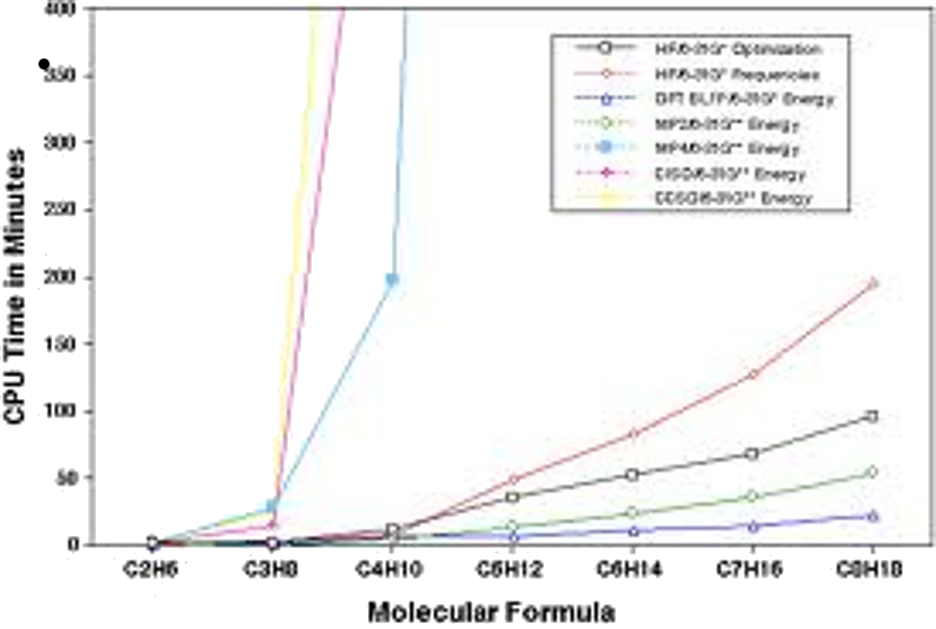
\includegraphics[width=1\linewidth]{cost.png} \\

With accurate but very expensive methods like the Coupled-Cluster (CC) method, each new digit in the energy may costs 10000 times more CPU time!

{\centering \textbf{{\color{green} 1 minute}  $\rightarrow$ {\color{orange} 1 week} $\longrightarrow$ {\color{red} 200 years}}}

 \vspace{1.25em}

Even one of the simplest approach, the Hartree-Fock (HF) method, scales conventionally as $\ensuremath{\mathcal{O}}(M^3)$.

This means that  choosing another molecule  that is 10 times larger than the current one increases the computational effort  by a factor of 1000!

 \vspace{1.25em}

Fortunately we benefit from  exciting improvements in  computer power over time nowadays mainly driven by the game and IT industry. (e.g. ENIAC vs PS3)

  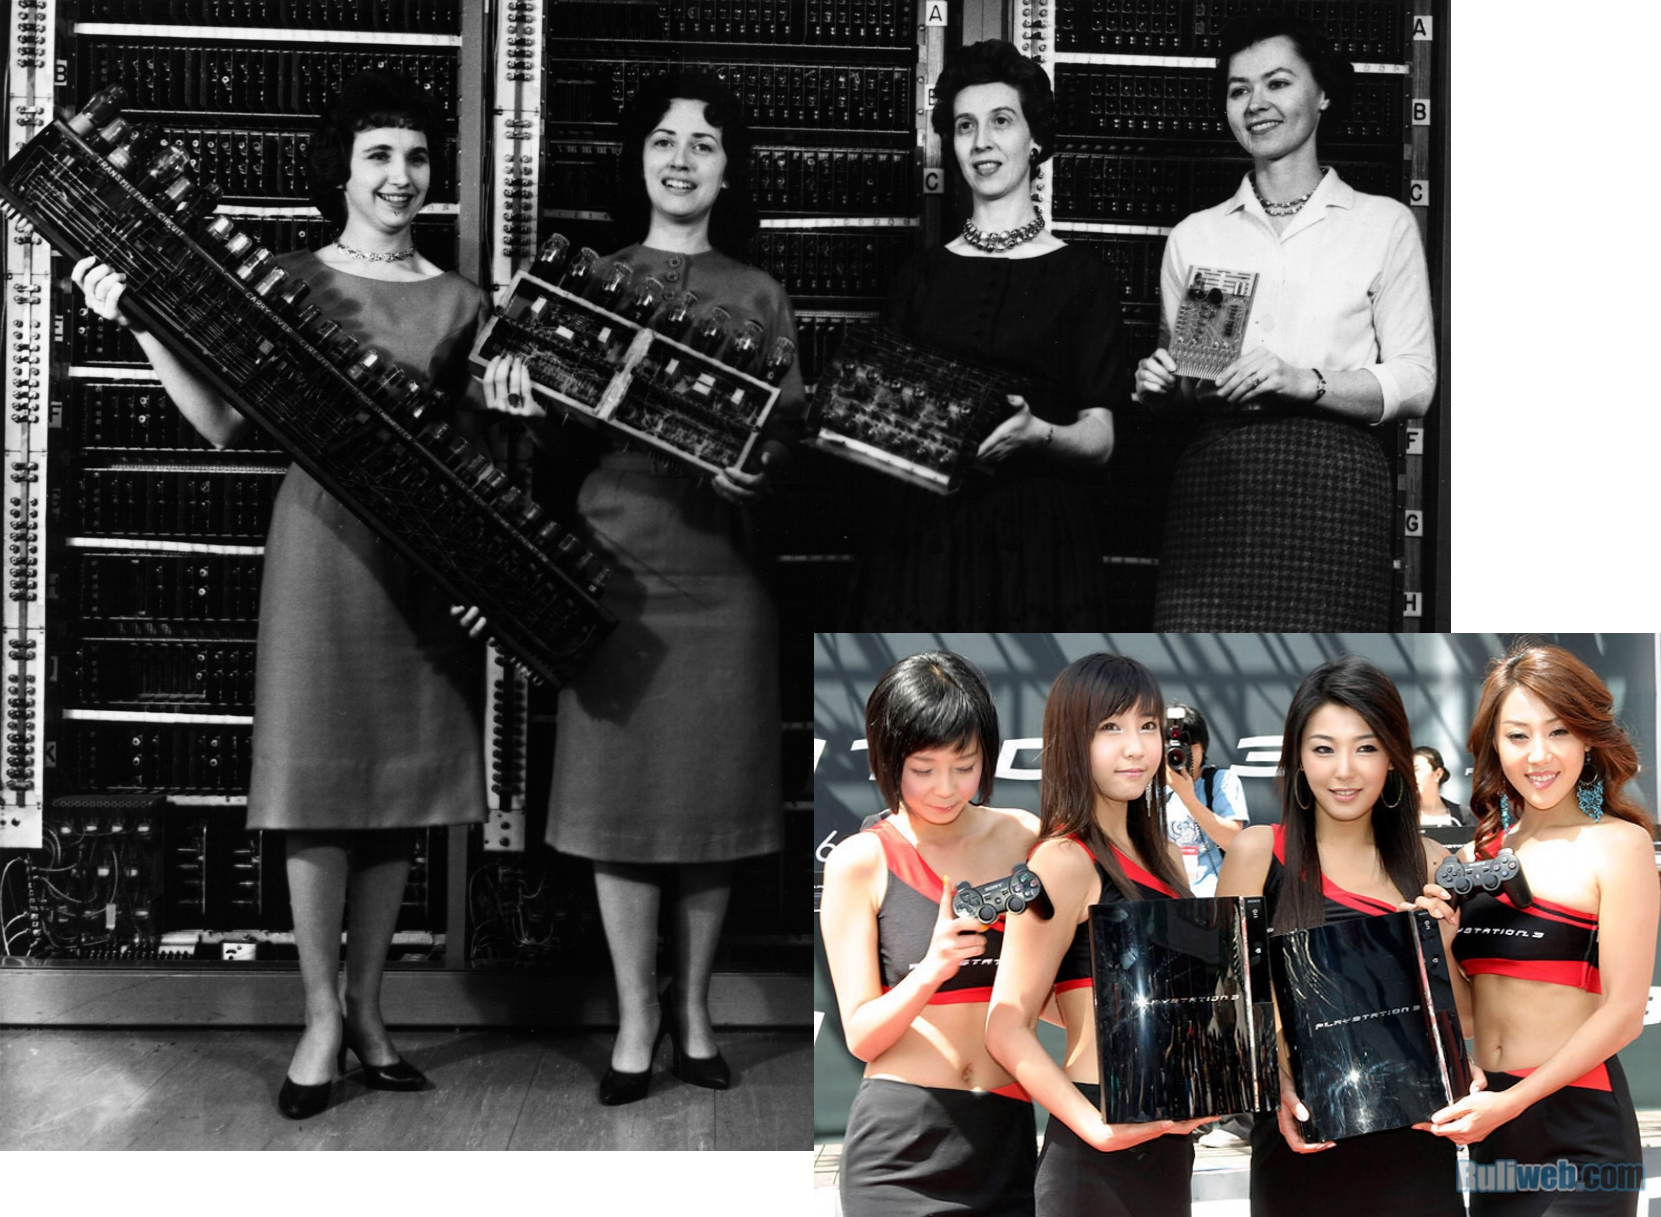
\includegraphics[scale=0.1]{eniacWomen_PS3Koreans.png} \\

Moore's law is still astonishingly valid over the last decades, predicting that computer speed might double every 1.5 years. Then in 15 years, the computers speed might be multiplied by about a factor 1000 ($2^{10}=1024$).

 \vspace{1.25em}

\textbf{Should we wait 15 years of hardware improvements to simulate molecules only 10 times larger within the same time frame?} 
\\
%While the biggest molecules we can simulate today are about a few hundreds of atoms, we won't be able to reach biomolecules soon only relying on hardware improvements.
% We really need to reduce the scaling behaviour of the methods in parallel of the progresses on hardware. 

   }


 %%%%%%%%%%%%%%%%%%%%%%%%%%%%%%%%%%%%%%%%%%%%%%%%%%%%%%%%%%%%%%%%%%%%%%%%%%%%%%
   \headerbox{Linear-Scaling}{name=linearscaling,column=2,row=0,span=1}{
 %%%%%%%%%%%%%%%%%%%%%%%%%%%%%%%%%%%%%%%%%%%%%%%%%%%%%%%%%%%%%%%%%%%%%%%%%%%%%%
%  \vspace{1.25em}
  In order to reach the size of biomolecules, \textbf{the scaling behaviour of the QM  methods has to be reduced,} optimally to scale linearly with system  size.

The  idea is to exploit the sparsity of different matrices involved in the calculations (e.g. overlap and eri matrices).

% \hspace{3em}
 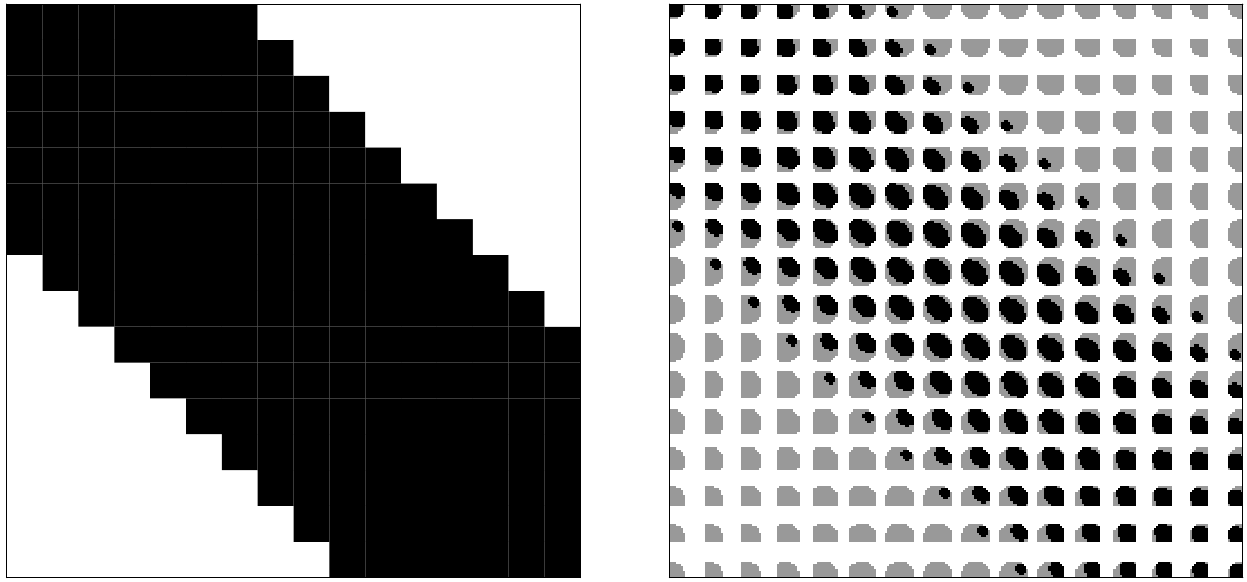
\includegraphics[width=1\linewidth]{sparsity_S_ERI.png}

 \vspace{1.25em}
LS techniques are already successfully developed for few methods (SCF methods): to compute the energy of a system, to optimize their geometry and to get some  response properties that can be compared to experimental results (such as vibrational frequencies, NMR shieldings).  

%% \begin{itemize}
%%  \item Fock-type matrices construction \\
%%    (intg. screening, CFMM, LinK),

%%  \item avoiding  diagonalization steps  \\
%% (Density matrix-based SCF),

%%  \item the energy gradient,

%%  \item response properties to perturbation\\
%% (vib. freq., NMR shieldings).

%% \end{itemize}

The efficient evaluation of ``exact exchange in Fock-type matrices'', which is a pure quantum mechanical term, is particularly important to include for large molecular systems since without it, calculations typically fail to converge \\
(e.g. Insulin: 787 atoms).

%\hspace{3em}
%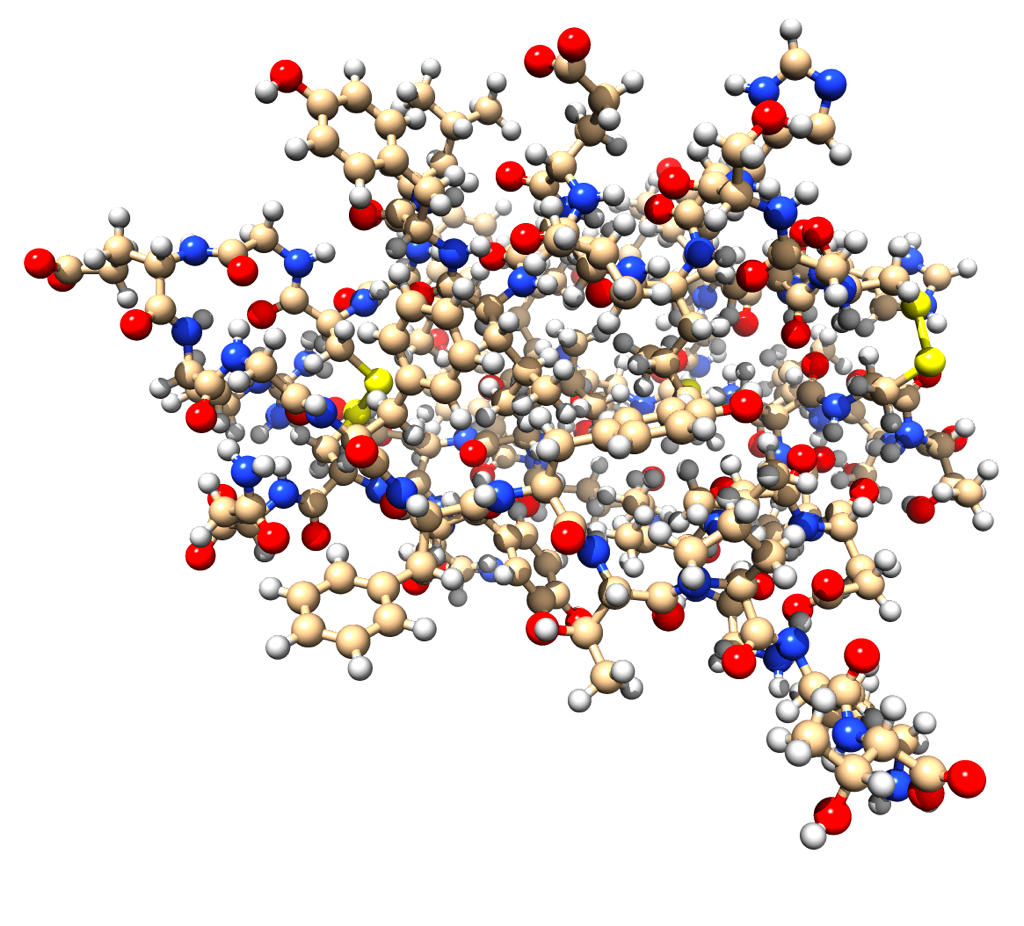
\includegraphics[width=0.3\linewidth]{insulin_TKJ.png}

Linear-scaling methods also perfectly combine with new computer architectures to allow  \textbf{massively parallel} calculations.

\hspace{5em}
 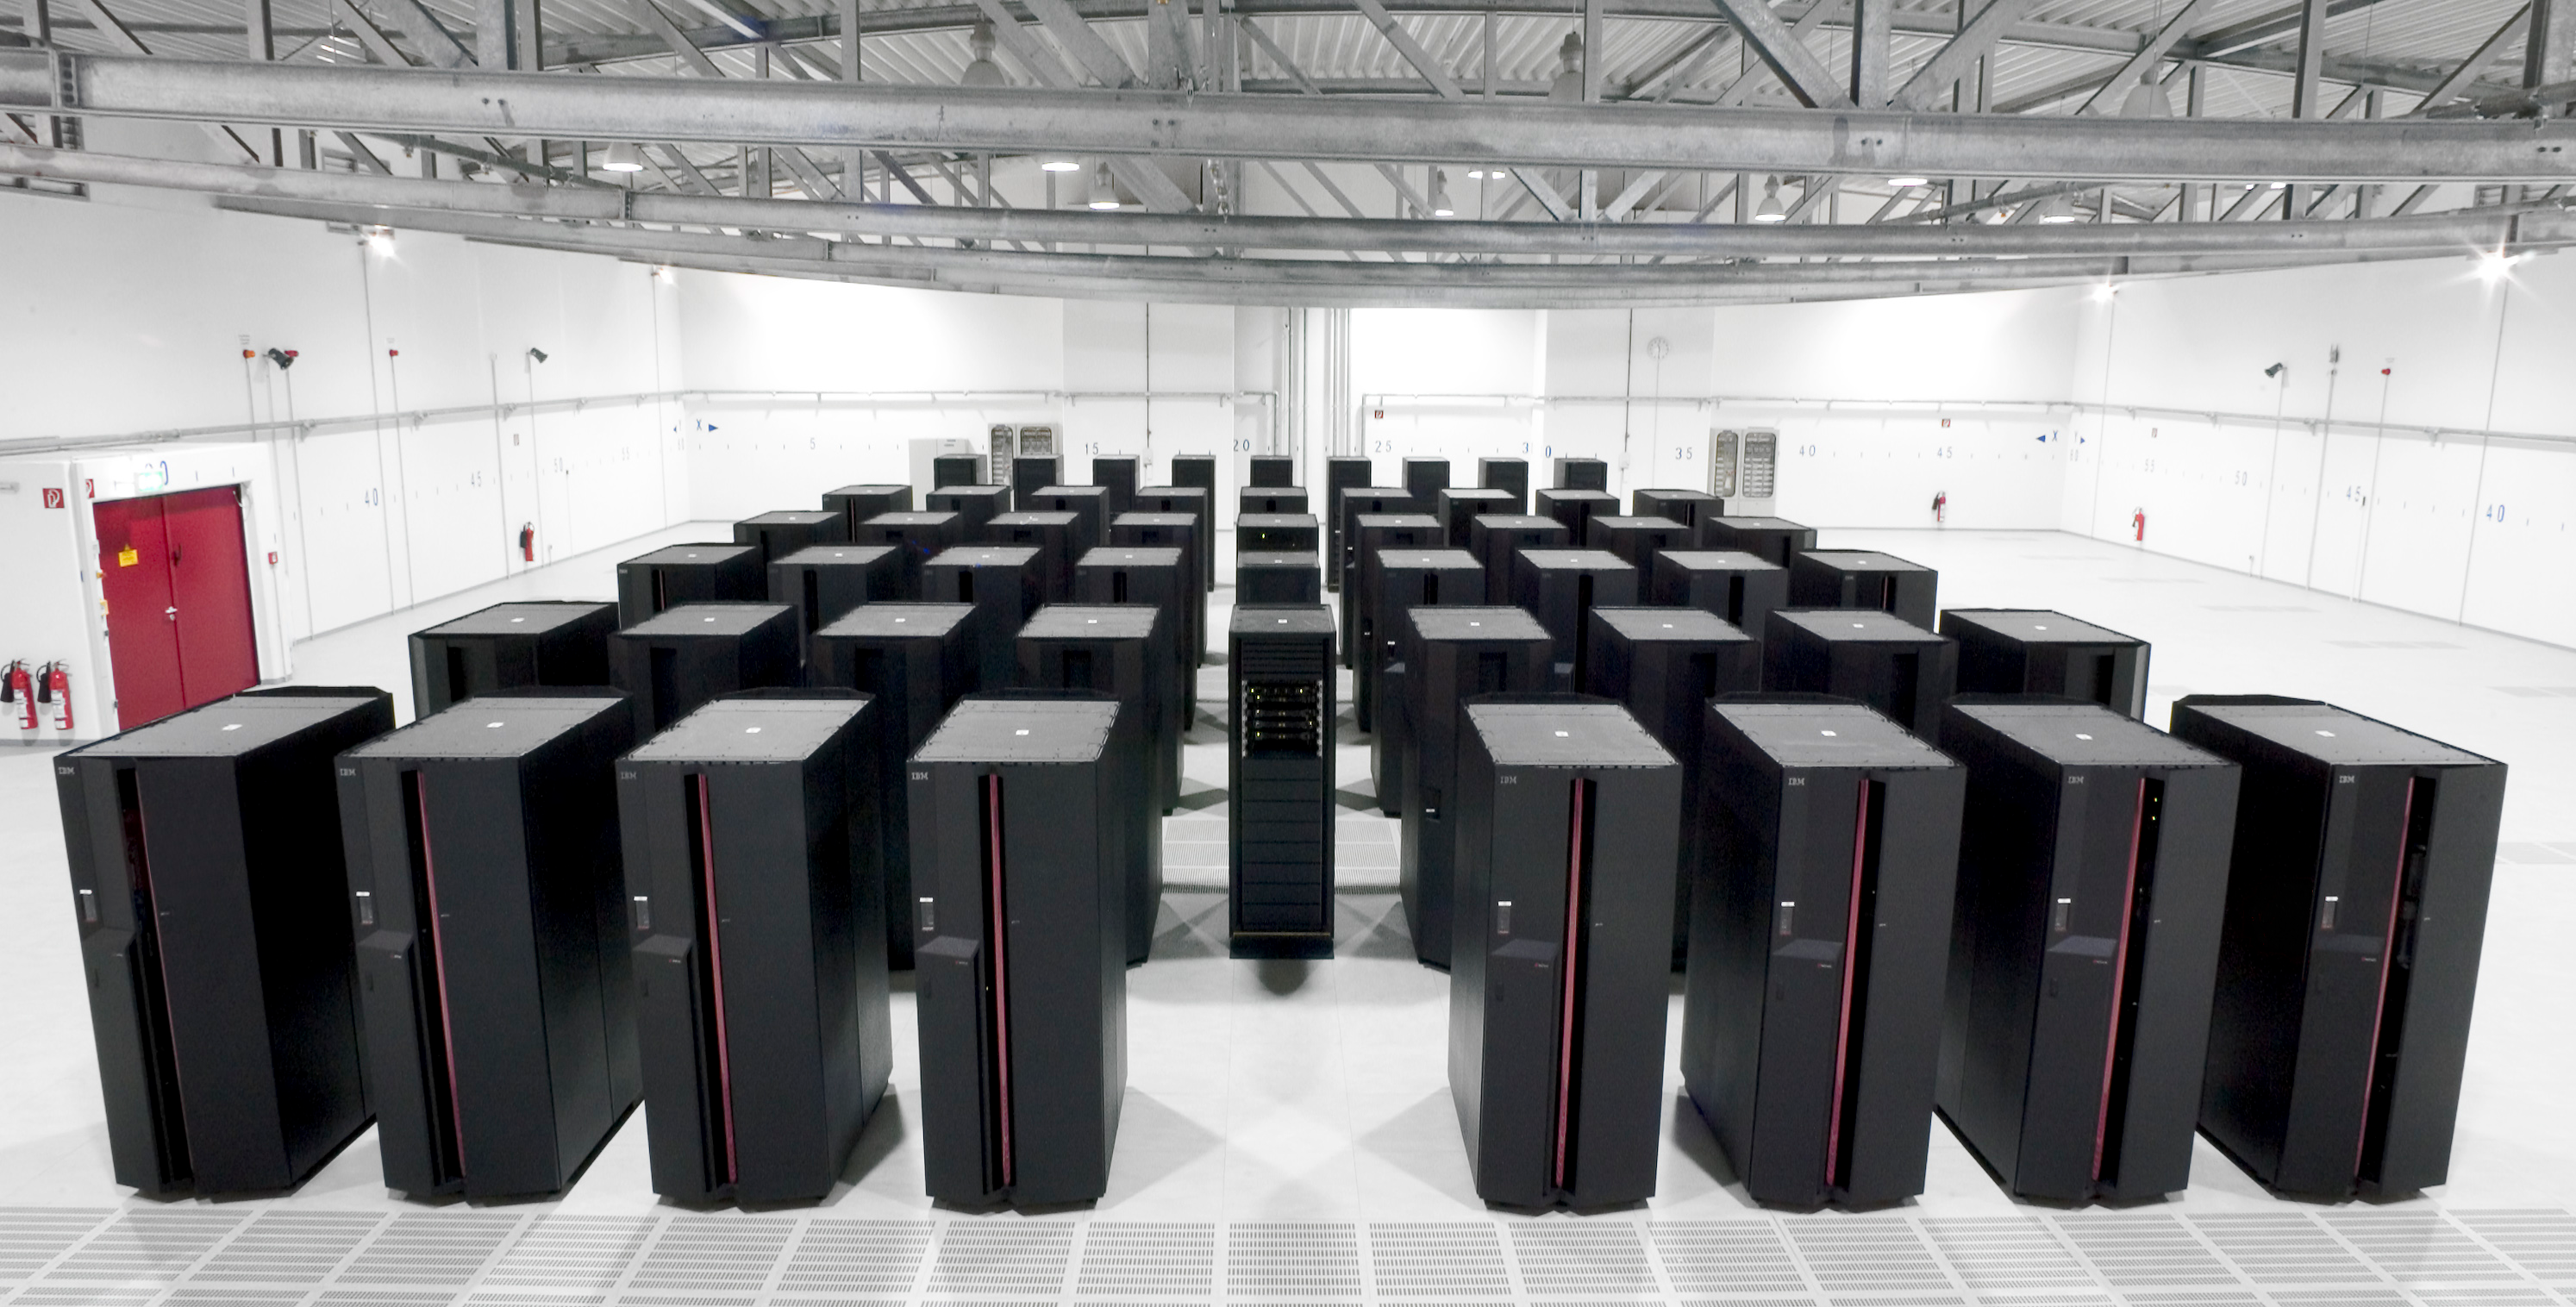
\includegraphics[width=0.7\linewidth]{ibm_supercomputer.png}

%\framebox[\textwidth][l]{%
%   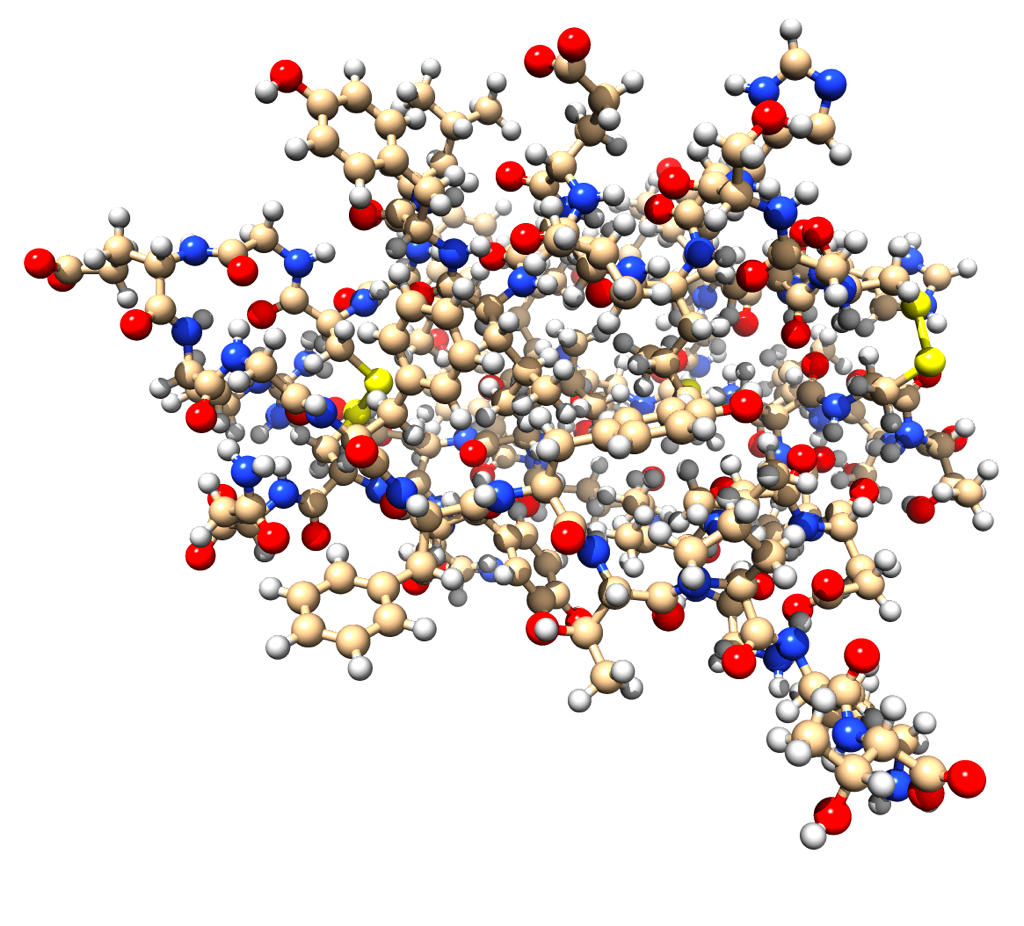
\includegraphics[width=0.3\linewidth]{insulin_TKJ.png}
%}


   }


%%  %%%%%%%%%%%%%%%%%%%%%%%%%%%%%%%%%%%%%%%%%%%%%%%%%%%%%%%%%%%%%%%%%%%%%%%%%%%%%%
%%    \headerbox{Our methods ...}{name=methods,column=2,row=0,span=1}{
%%  %%%%%%%%%%%%%%%%%%%%%%%%%%%%%%%%%%%%%%%%%%%%%%%%%%%%%%%%%%%%%%%%%%%%%%%%%%%%%%
%% %   \textbf{PARI:}
%% %One of the strongest approximation that can be made on 4-center 2-electron integrals, one of the most expensive and slow part of the calculations.
%%    }


 %% %%%%%%%%%%%%%%%%%%%%%%%%%%%%%%%%%%%%%%%%%%%%%%%%%%%%%%%%%%%%%%%%%%%%%%%%%%%%%%
 %%   \headerbox{References}{name=references,column=0,above=bottom}{
 %% %%%%%%%%%%%%%%%%%%%%%%%%%%%%%%%%%%%%%%%%%%%%%%%%%%%%%%%%%%%%%%%%%%%%%%%%%%%%%%
 %%     \smaller
     
 %%     \bibliographystyle{ieee}
 %%     \renewcommand{\section}[2]{\vskip 0.05em}
 %%       \begin{thebibliography}{1}\itemsep=-0.01em
 %%       \setlength{\baselineskip}{0.4em}

 %%       \bibitem{pari}
 %%       P.~Merlot, T.~Kj{ae}rgaard, T.~Helgaker, R.~Lindh, F.~Aquilante, S.~Reine, T.~Bondo Pedersen
 %%       \newblock The pari-atomic resolution-of-the-identity approximation for four-center two-electron integrals
 %%       %\newblock In {\em JCP}, 2012.
 %%       \newblock {\em (not yet published)} , 2012.

 %%       \end{thebibliography}
 %%   }

   %%%%%%%%%%%%%%%%%%%%%%%%%%%%%%%%%%%%%%%%%%%%%%%%%%%%%%%%%%%%%%%%%%%%%%%%%%%%%%
   \headerbox{Check This Out!}{name=contacts,column=0,above=bottom}{
     %%%%%%%%%%%%%%%%%%%%%%%%%%%%%%%%%%%%%%%%%%%%%%%%%%%%%%%%%%%%%%%%%%%%%%%%%%%%%%
     \smaller
     \smaller
     \begin{tabular}{rll}
       \multirow{3}{*}{ 
\includegraphics[width=0.22\linewidth]{apollon-rod.png} } & \multirow{3}{*}{ 
\includegraphics[width=0.22\linewidth]{qrcode_webLink.png} } & Center for        \\
          &                             & Theoretical \&  \\
          &                             &   Computational \\
          &                             &   Chemistry      \\
          &                             & \mbox{\url{www.CTCC.no}}   \\
       \end{tabular}
   }


   %%%%%%%%%%%%%%%%%%%%%%%%%%%%%%%%%%%%%%%%%%%%%%%%%%%%%%%%%%%%%%%%%%%%%%%%%%%%%%
   \headerbox{Acknowledgements}{name=ack,column=2,above=bottom}{
     %%%%%%%%%%%%%%%%%%%%%%%%%%%%%%%%%%%%%%%%%%%%%%%%%%%%%%%%%%%%%%%%%%%%%%%%%%%%%%
     \smaller
     %% This work is receiving support from the Norwegian Research Council, and computer resources 
     %% are provided by the Norwegian Metacenter for Computational Science (NOTUR) through the Center for Theoretical and Computational Chemistry (CTCC) at the University of Oslo.

     This work is receiving support from the Center for Theoretical and Computational Chemistry (CTCC) at the University of Oslo.
   }
   

 %%%%%%%%%%%%%%%%%%%%%%%%%%%%%%%%%%%%%%%%%%%%%%%%%%%%%%%%%%%%%%%%%%%%%%%%%%%%%%
   \headerbox{Challenges}{name=discussion,column=2,row=0,span=1,below=linearscaling,above=ack}{
 %%%%%%%%%%%%%%%%%%%%%%%%%%%%%%%%%%%%%%%%%%%%%%%%%%%%%%%%%%%%%%%%%%%%%%%%%%%%%%
There is still great need for developing and improving linear-scaling methods.

Many molecular properties remain without linear-scaling development, small ``homo-lumo'' gaps affect a lot the performances and the flexibility of large molecules emphasizes the importance of very fast and cheap dynamics simulations. 
   }


%%  %%%%%%%%%%%%%%%%%%%%%%%%%%%%%%%%%%%%%%%%%%%%%%%%%%%%%%%%%%%%%%%%%%%%%%%%%%%%%%
%%    \headerbox{Training + Testing Data}{name=data,column=0,above=references,below=abstract}{
%%  %%%%%%%%%%%%%%%%%%%%%%%%%%%%%%%%%%%%%%%%%%%%%%%%%%%%%%%%%%%%%%%%%%%%%%%%%%%%%%
%% %   \includegraphics[width=0.2\linewidth]{09_6m_masked}%
%% %   \includegraphics[width=0.2\linewidth]{33_4m_masked}%
%%    %\includegraphics[width=0.2\linewidth]{22_3f_masked}
%%    $\dots$\\
%%    The model was trained from 456 images from the IMM and XM2VTS datasets using
%%    120 landmarks. Get the landmarks, model, and source code at:\\
%%    \mbox{\url{www.cs.unibas.ch/personen/amberg_brian/aam/}}
%%    }

 %%%%%%%%%%%%%%%%%%%%%%%%%%%%%%%%%%%%%%%%%%%%%%%%%%%%%%%%%%%%%%%%%%%%%%%%%%%%%%

 %%   \headerbox{Tracking 5000 frames with a general model}{name=tracking,column=2,span=2,below=speed,above=bottom}{
 %% %%%%%%%%%%%%%%%%%%%%%%%%%%%%%%%%%%%%%%%%%%%%%%%%%%%%%%%%%%%%%%%%%%%%%%%%%%%%%%
 %%   \vspace{-1.2em}
 %%   \begin{multicols}{2}
 %%   {\textbf{Our algorithm makes fast and robust tracking possible.}
 %%     We compare face tracking under natural motion, using \ICIA{},
 %%     \LinCoDe{} and \CoDe{}. The original \ICIA{} fails
 %%     immediately with this large model and new face data. Substituting the orthonormal
 %%     incremental warp for the original \ICIA{} warp, the algorithm still loses track
 %%     very early, whereas \LinCoDe{} and \CoDe{} can track much
 %%     further. Finally, adding regularisation to all algorithms, \ICIA{} still
 %%     loses track completely after approximately 500 frames and does not recover
 %%     the local deformations accurately. In contrast \CoDe{} now tracks the full
 %%     5000 frame sequence without reinitialization, and \LinCoDe{} tracks for 2500 frames.}
   
 %%   The same training dataset was used for both tracking experiments. The
 %%   training data was aquired with different camera and light settings from
 %%   different subjects.
 %%   \end{multicols}
 %%   }





\end{poster}%
%
\end{document}
